\documentclass[border=5pt]{standalone}
\usepackage[T1]{fontenc}
\usepackage{lmodern}
\usepackage{pgfplots}
\usepgfplotslibrary{groupplots}
\usetikzlibrary{calc}
\pgfplotsset{compat=1.18}
\definecolor{hostblue}{HTML}{2166AC}
\definecolor{recomputered}{HTML}{B2182B}
\begin{document}
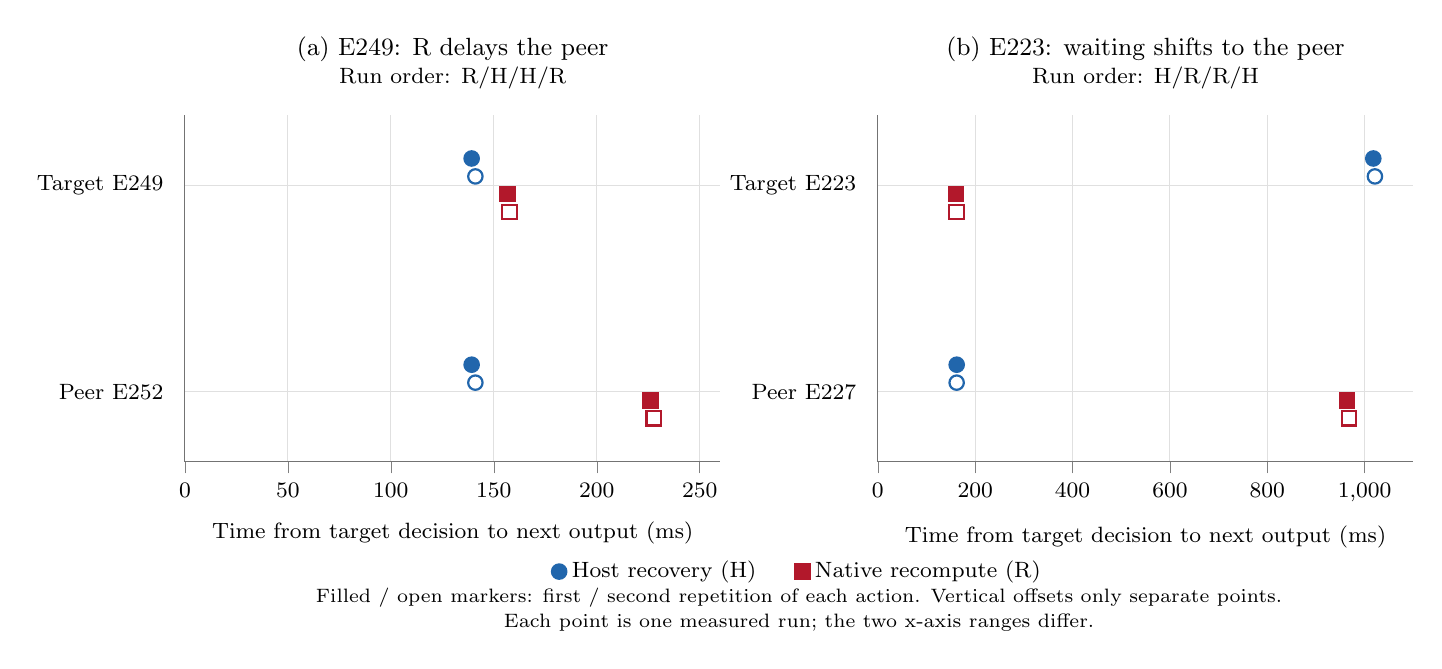
\begin{tikzpicture}
\begin{groupplot}[
 group style={group size=2 by 1,horizontal sep=2.0cm},
 width=6.8cm,height=4.4cm,scale only axis,
 xmin=0,ymin=-0.34,ymax=1.34,
 ytick={0,1},ytick style={draw=none},
 xlabel={Time from target decision to next output (ms)},
 xlabel style={font=\fontsize{8}{9}\selectfont,yshift=-2pt},
 tick label style={font=\fontsize{8}{9}\selectfont},
 title style={font=\fontsize{9}{11}\selectfont,align=center},
 axis x line*=bottom,axis y line*=left,
 axis line style={black!55},xmajorgrids=true,ymajorgrids=true,
 grid style={black!12},tick align=outside,
 legend style={draw=none,font=\fontsize{8}{9}\selectfont,/tikz/every even column/.append style={column sep=12pt}},
 legend columns=2,
 every axis plot/.append style={only marks,mark size=2.6pt,line width=0.8pt},
]
\nextgroupplot[legend to name=recoverylegend,xmax=260,xtick={0,50,100,150,200,250},yticklabels={Peer E252,Target E249},title={(a) E249: R delays the peer\\[-1pt]{\footnotesize Run order: R/H/H/R}}]
\addplot[color=hostblue,mark=*] coordinates {(139.232065529,1.130) (139.232065529,0.130)};
\addlegendentry{Host recovery (H)}
\addplot[color=hostblue,mark=o,forget plot] coordinates {(141.042841598,1.043) (141.042841598,0.043)};
\addplot[color=recomputered,mark=square*] coordinates {(156.625552103,0.957) (226.086916402,-0.043)};
\addlegendentry{Native recompute (R)}
\addplot[color=recomputered,mark=square,forget plot] coordinates {(157.593453303,0.870) (227.640045807,-0.130)};
\nextgroupplot[xmax=1100,xtick={0,200,400,600,800,1000},yticklabels={Peer E227,Target E223},title={(b) E223: waiting shifts to the peer\\[-1pt]{\footnotesize Run order: H/R/R/H}}]
\addplot[color=hostblue,mark=*,forget plot] coordinates {(1017.841638997,1.130) (162.005173042,0.130)};
\addplot[color=hostblue,mark=o,forget plot] coordinates {(1021.209083498,1.043) (161.907525733,0.043)};
\addplot[color=recomputered,mark=square*,forget plot] coordinates {(160.731604323,0.957) (963.786507025,-0.043)};
\addplot[color=recomputered,mark=square,forget plot] coordinates {(161.774270236,0.870) (967.967975885,-0.130)};
\end{groupplot}
\node[anchor=north] at ($(group c1r1.south west)!0.5!(group c2r1.south east)+(0,-1.0cm)$)
 {\pgfplotslegendfromname{recoverylegend}};
\node[anchor=north,font=\fontsize{7.5}{9}\selectfont,align=center]
 at ($(group c1r1.south west)!0.5!(group c2r1.south east)+(0,-1.48cm)$)
 {Filled / open markers: first / second repetition of each action. Vertical offsets only separate points.\\
  Each point is one measured run; the two x-axis ranges differ.};
\end{tikzpicture}
\end{document}
